%%% Article Template
%%% Set Document layout
\documentclass[final, 11pt]{article}


%%%%%%%%%% Set Name, Subject, Date ...
\newcommand{\toppic}{Vektoren}
\newcommand{\mytitle}{MathMeth 1 Zusammenfassung}
\newcommand{\workingDate}{27.12.2022}
\newcommand{\userName}{Vektoren, Matzitzen, Integrale, DGL, Nabla,...}
%%
\usepackage{options}
 
%%%%%%%%%% Begin the document
\begin{document}  
\begin{center}
    {\textbf {\huge \mytitle}}\\[5mm]   % titel
    {\large \userName} \\[5mm]          % User Name
    \workingDate\\                      % Working Date
\end{center} %%%%%%%%%% Titel %%%%%%%%%%%%%%

%%
\section{Begriffe / Zeichen / Rechenregeln}  
\begin{center}
    \begin{tblr}{ll}
        \textbf{Symbol}         & \textbf{Bedeutung} \\ \hline[1.5pt]
        $R$                    & Relation \\\hline
        $\in/ \notin$          & Element / kein Element von \\\hline
        $\forall / \nexists$   & für alle / für kein \\\hline
        $\exists$              & Existenzquantor, mindestens ein \\\hline
        $\exists !$            & Anzahlquantor, genau ein \\\hline
        $A \subset B$          & echte Teilmenge, $a \in A \land a,b \in B:\exists b\notin A$\\ \hline
        $A \subseteq B$             & Teilmenge $a \in A \land a,b \in B$ \\\hline
        $]1,3[$, $(1,3)$       & $1<x<3$ \\\hline
        $[1,3]$                & $1\leq x \leq 3$ \\\hline
        $\Rightarrow$          & genau dann wenn \\\hline
        $\Leftrightarrow$      & aus Aussage A folg B und umgekehrt \\\hline
        $\rightarrow$          & Abbildungsvorschrift für Mengen \\\hline
        $\mapsto$              & Abbildungsvorschrift für Elemente \\\hline
        $\circ$                & Komposition / Verkettung von Funktionen \\\hline
        $\land\ /\ \lor$       & und / oder \\\hline
        Lemma                  & Hilfssatz \\\hline
        $\overline{z}, \ z^*$  & konjungiert komplexe Zahl \\\hline
        $\preccurlyeq$         & beliebiges Symbol \\\hline
        $\stackrel{?}{=}$      & zu zeigen \\\hline
        $\stackrel{!}{=}$      & soll erfüllt sein um ... zu zeigen \\\hline
        $:=, \equiv$           & definiere \\\hline
        $\cup,\cap, /$         & Vereinigung, Durchschnitt, Subtrahiert \\\hline
        disjunkt               & $A \cap B = \{\}$ \\\hline
        infimum \\\hline
        supremum \\\hline
        notwendiges Kriterium & muss immer erfüllt sein, reicht aber nicht aus\\ \hline
        hinreichendes Kriterium & wenn erfüllt dann ... \\ \hline
        Nullfolge  &   $(a_k)_k$ ist eine Nullfolge wenn $\lim_{k\to\infty}a_k=0$\\ \hline
        surjektiv & $\forall y \in Y : \exists \  x \in X:f(x)=y$ \ref{subs:surjektivitaet}\\ \hline
        injektiv &$\forall x_1,x_2 \in X:f(x_1)=f(x_2) \Rightarrow x_1=x_2$   \ref{subs:injektivitaet}\\ \hline
        bijektiv & $\forall y \in Y : \exists ! \  x \in X:f(x)=y$\ref{subs:bijektivitaet}\\ \hline
        beschränkte Folge & $\exists b,c : \forall n: b<a_n<c$ \\ \hline
        nach oben beschränkte Folge &  $\exists b: \forall n: a_n<b$\\ \hline
        nach unten beschränkte Folge &  $\exists b: \forall n: b<a_n$\\ \hline
    \end{tblr}
\end{center}




%%%%
\section{Reihen und Folgen}
\begin{description}
    \item[\textbf{Definition:}] Eine Reihe ist eine Partialsumme einer Folge $(p_n)_n = \left(\sum\limits_{i=0}^{n}a_i \right)_n$, $p_n$... Reihe, $a_i$... Folge\\
    \item[\textbf{harmonische Reihe:}] $\sum\limits_{k=1}^{\infty}\frac{1}{k}$ ist divergent\\
    \item[$\sum\limits_{k=1}^{\infty}\frac{1}{k^r}$] konvergiert für $r\geq 2$\\
\end{description}




\subsection{Konvergenzkriterien}

\textbf{Definition Konvergenz:} \\

\textbf{Definition absolute Konvergenz:} \\$\sum\limits_{k=1}^{\infty}\frac{1}{k}$ 

\subsubsection{Minoranten- Majoranten Kriterium}

\subsection{Quotientenkriterium}

\subsection{Wurzelkriterium}

\section{Vektoren}
\begin{description}
    \item [\textbf{Einheitsvektor:}] Jeder Vector mit Betrag 1. $\vec{e_x}=\frac{\vec{x}}{|\vec{x}|}$\\

    \item[\textbf{Skalarprodukt:}] $\vec x \cdot \vec{y} = x_1\cdot y_1 + x_2\cdot y_2 + x_3\cdot y_3 = |\vec{x}|\cdot|\vec{y}|\cdot \cos(\varphi)$\\
    Null, wenn $\vec x $ und $\vec y $ normal aufeinander stehen. Gibt die gemeinsame Länge von in eine  Richtung an.\\
    \textbf{Schwarzsche Ungleichung:} $|x\cdot y|\leq |x|\cdot |y|$\\
    
    \item[\textbf{Kreuzprodukt:}] $z = \vec x \times \vec y  = 
    \begin{pmatrix}
        x_2y_3-x_3y_2\\
        x_3y_1-x_1y_3\\
        x_1y_2-x_2y_1\\
    \end{pmatrix}$\\
    
    $z$ steht \textbf{senkrecht} auf $\vec x $ und $\vec y $\\
    $A = |\vec x \times \vec y |$... Fläche des von $\vec x $ und $\vec y $ aufgespannten Parallelogramms.\\

    \item[\textbf{Winkel zwischen Vektoren:}]  $\varphi = \arccos \frac{\vec x \cdot \vec y }{|\vec{\vec x }|\cdot |\vec y |}$\\
    
    \item[\textbf{Spatprodukt:} ] Flälche zwischen 3 Vektoren, $V = |\vec a \times \vec b |\cdot |\vec c | \cdot cos \varphi = (\vec a \times \vec b )\cdot \vec c $\\
    
    \item[\textbf{Projektion von x in Richtung y:}] $x_y=\vec{e_y}\cdot \vec{x} \cdot \vec{e_y}=\frac{\vec{y}\cdot \vec{x}}{|\vec{y}|^2} \cdot \vec{y}$\\
    $\vec{e_y}\cdot \vec{x} = |\vec{e_y}|$ gibt die Länge von x in Richtung y an. Multipliziert mit $\vec{e_y}$ um einen Vektor zu erhalten.
    

\end{description}
 

\section{Komplexe Zahlen und Funktionen}
\subsection{rechnen mit komplexen Zahlen}
$z = a +ib = |z|e^{i \varphi} \qquad z_1 = a_1+ib_1 \qquad z_2 = a_2+ib_2$\\
$z^*$... konjungiert komplex ($z=a+ib \qquad z^*=a-ib$)\\

\textbf{Betrag:} $|z| = \sqrt{a^2+b^2} = \sqrt{z\cdot z^*}$\\
\textbf{Winkel:} $\varphi _z = \text{arctan}(\frac{b}{a})$\\

\textbf{Komponentenform:} $z=a+ib$

\textbf{Polarform:} $z = |z|e^{i\varphi _z}$\\

\textbf{Addition:} $z_1 \pm z_2 = (a_1 \pm a_2) + i(b_1 \pm b_2)$\\

\textbf{Multiplikation:} $z_1 \cdot z_2 = (a_1 + ib_1) \cdot (a_2 + ib_2) = (a_1a_2 - b_1b_2) + i(a_1b_2 + a_2b_1)$\\
$z_1\cdot z_2 = |z_1|\cdot |z_2|e^{i(\varphi _{z_1} +\varphi _{z_2})}$\\


\textbf{Division:} $\frac{z_1}{z_2}=\frac{z_1}{z_2} \cdot \frac{z_1^*}{z_2^*} = \frac{(a_1a_2+b_1b_2)+i(a_2b_1-a_1b_2)}{a_2^2+b_2^2}$\\
$z_1 \cdot z_2 = \frac{|z_1|}{|z_2|}e^{i(\varphi _{z_1} -\varphi _{z_2})}$\\

\textbf{Wurzel} $\sqrt{z} = \sqrt{|z|}\cdot e^{i \frac{\varphi +k\cdot 2\pi}{n}} \quad n \in [0,...,n-1]$\\
Da n verschiedene Lösungen herauskommen müssen, wird zu $\varphi, k*2\pi$ addiert(verändert die Funktion nicht). Beim ziehen der n-ten Wurzel wird der Exponent mit $\frac{1}{n}$ multipliziert.

\subsection{Differenzierbarkeit komplexer Funktionen (Cauchy-Riemannschen Differenzialgleichungen)}

Komplexe Funktionen sind differenzierbar, wenn die Chauchy-Riemannschen Dgl erfüllt sind.\\

$z=u(x,y) + iv(x,y)\qquad f(z) = u(x,y) + iv(x,y)$\\

\[\text{Cauchy-Riemannschen Dgl:}\qquad \frac{\partial u(x,y)}{\partial x} = \frac{\partial v(x,y)}{\partial y} \quad \text{und } \frac{\partial u(x,y)}{\partial y} = - \frac{\partial v(x,y)}{\partial x} \]

%%%%
\section{Integrieren / Differenzieren}
%%
\subsection{Differenzieren}
Berechnung der Steigung der Funktion. ($\frac{dy}{dx}$)

\begin{center}
	\captionsetup{type=figure}
	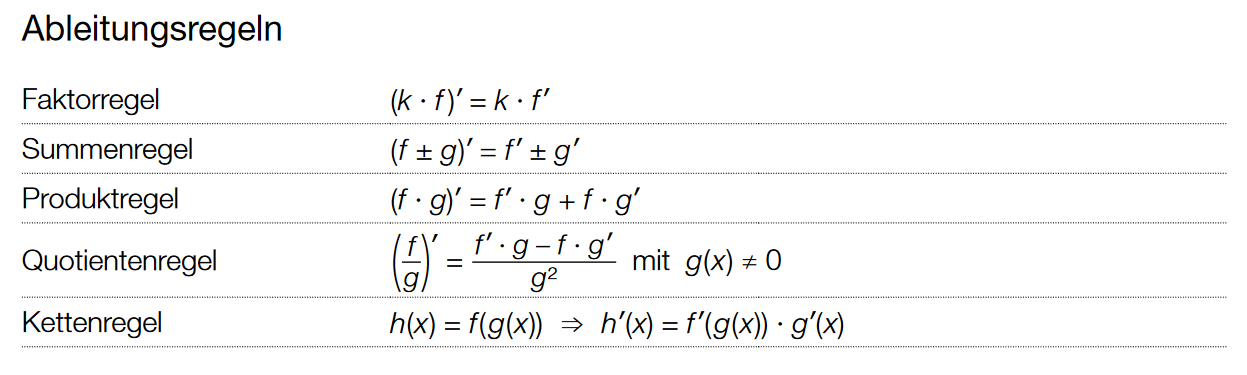
\includegraphics[width=0.9\linewidth]{pictures/Ableitungsregeln_Formelsammlung_Matura}
	\caption{Formelsammlung~\cite[S. 13]{Formelsammlung_BHS}}
	\label{fig:ableitungsregeln}
\end{center}



%%
\subsection{Integrieren}
Berechnung der Fläche zwischen der Funktion und der X-Achse. ($dx \cdot dy$)
\begin{enumerate}
	\item Man bestimme eine Stammfunktion $F(x)$ zum Integranden $f(x)$
	\item Mit dieser Stammfunktion berechnet man die Differnenz $F(b)-F(a)$
\end{enumerate}
\[\int\limits_a^b f(x) dx = \left . \left[F(x)\right] \right | _a^b = F(b)-F(a)\]

\textbf{unbestimmtes Integral:}
Das unbestimmte Integral gibt zu einer Funktion die Menge aller Stammfunktionen an.

%
\subsubsection{Grundintegrale}

\begin{center}
	\captionsetup{type=figure}
	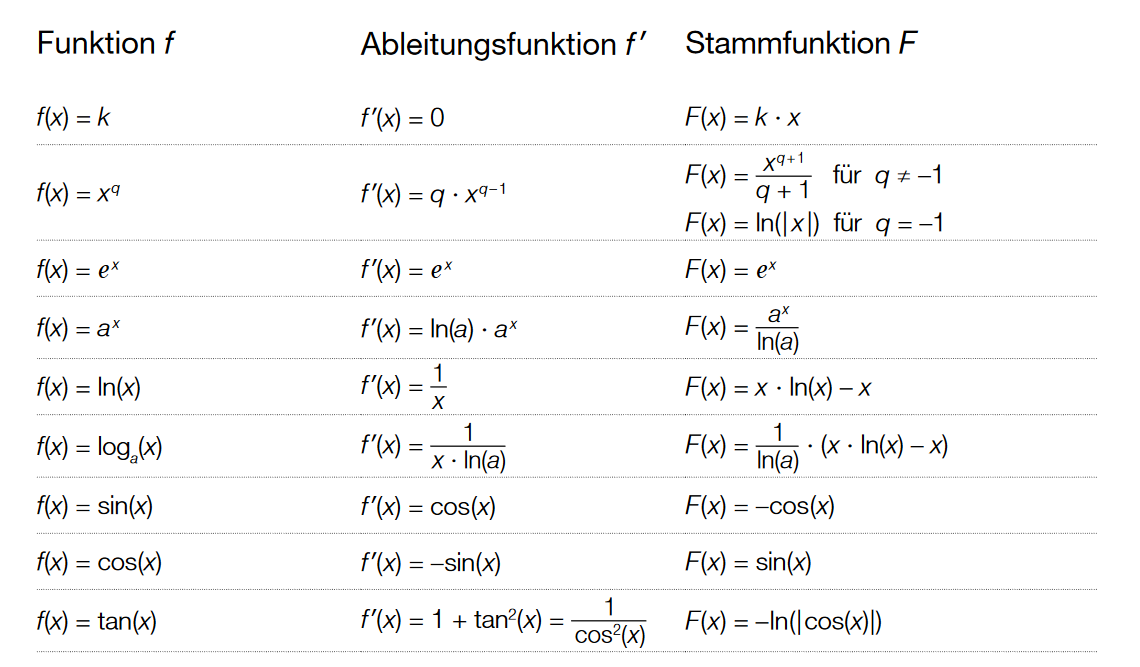
\includegraphics[width=0.9\linewidth]{pictures/Grundintegrale_Formelsammlung_BHS}
	\caption{Grundintegrale \cite[S. 13]{Formelsammlung_BHS}}
	\label{fig:grundintegrale}
\end{center}

%%
\subsubsection{Substituieren}
Bei Funktionen in Funktionen immer die innere Funktion substituieren.
Substitution wird gemacht, damit man die x wegkürzen kann. 
Wenn man eine substituierte Funktion integriert, müssen alle x weg sein! Integreieren nach u ist mit x in der Gleichung \textbf{nicht möglich}!!!\\
\[\int f\left[g(x)\right] dx = \int f(u) \frac{du}{g'(x)}\]

\subsubsection{Partielle Integration:}
\[\int u(x)\cdot v'(x)dx = u(x)\cdot v(x)-\int u(x)'\cdot v(x)dx\]

\subsubsection{Phönix Integral:}
$f(x)= \int g(x)h(x)dx$\\

Wenn weder $g(x)$ noch $h(x)$ beim Ableiten einfacher wird, sondern gleich bleibt oder sich wiederholt (Bsp.: $e^x, sin(x), cod(x)...$) wird solange partiell integriert, bis im Integral-Teil vom partiellen Integrieren die Ausgangsfunktion steht. Die beiden gleichen Integrale werden auf eine Seite gebracht und umgeformt bis $\int g(x)h(x)dx = ... $ dasteht.


%%
\subsection{Integrieren über den Betrag}
Beim Integrieren über einen Betrag muss die Funktion an jedem Nulldurchgang (falls vorhanden) aufgeteilt und integriert. Die negativen Stellen müssen in die Summe negativ eingehen.
Bsp.: $\int\limits_{0}^{e}|ln(x)| = |x*(ln(x)-1)|\big|_{0}^{e} = -x*(ln(x)-1)\big|_{0}^{1} + x*(ln(x)-1)\big|_{1}^{e}$ 
$\alpha$

%%%%
\subsection{Uneigentliche Integrale}
Ein Integral existiert, jedoch sind die Integrationsgrenzen nicht beschränkt.\\
\textbf{Fall 1:} Eine Grenze des Integrals ist $\infty$.
\[\int\limits_a^{\infty}f(x)dx = \lim \limits_{\lambda \to \infty}\int\limits_a^{\lambda}f(x)dx\]

\textbf{Fall 2:}
Eine Polstelle von f(x) liegt im zu integrierenden Bereich. Ist der Grenzwert des Integrals für $\lambda \to 0$ vorhanden, wird das uneigentliche Integral \textbf{konvergent} genannt, andernfalls heißt es \textbf{divergent}.\\
\textbf{Bsp.:} b ist Polstelle von f(x)\\
\[\int\limits_a^b f(x)dx=\lim\limits_{\lambda \to 0}\int\limits_a^{b-\lambda}f(x)dx\]
\textbf{Bsp.:} $c$ ist Polstelle von $f(x)$ mit $a<c<b$
\[\int\limits_a^b f(x) dx = \lim\limits_{\lambda \to 0}\int\limits_a^{c-\lambda}f(x)dx + \lim\limits_{\mu \to 0}\int\limits_a^{c-\mu}f(x)dx\]


%%%%
\subsection{Kurvenintegrale:}
Beim klassischen eindimensionalen Riemann- Integral integriert man über ein Intervall $[a,b]$ der reellen Achse.\\
Beim Kurvenintegral werden die integrationsbereiche als Kurven $C$ im $\mathbb{R}^n$ betrachtet.\\
\textbf{Kurvenintegral 1. Art:} Eine \textbf{reellwertige} Funktion $f:\mathbb{R}^n \ to \mathbb{R}$ wird über eine Kurve C integriert.\\
Es wird ein skalares Feld über eine Kurve integriert. Es kann zur berechnung der Länge einer Kurve sowie zur Berechnung linienhafter Ladungs/Masseverteilungen dienen.\\
\textbf{Kurvenintegral 2. Art (Arbeitsintegral):} Ein \textbf{Vektorfeld} wird über eine Kurve $C$ integriert. Dient zur Berechnung der nötigen Arbeit, um eine Masse/Ladung in einem Kraftfeld längs einer Kurve zu bewegen.\\

\textbf{Bogenelement:} $|\gamma'(t)dt|$\\

\subsubsection{Kurvenintegral 1. Art}
Für eine stückweise stetige Funktion $f:\mathbb{R}^n \to \mathbb{R}$ ist das Kurvenintegral von $f$ längs $\vec{\gamma}$: 
$$J=\int\limits_{\vec{\gamma}} fds = \int\limits_{t_a}^{t_e}f(\vec{\gamma} (t))\cdot |\dot{\gamma}(t)|dt$$

\textbf{Bsp.:} Bogenlänge $s(t)$ des Kurvenstücks $[t_a,t_e]$ der Kurve $C$:
\[s(t)=\int\limits_{t_a}^{t_e}\dot{\vec{\gamma}}(t)|dt= \int\limits_{t_a}^{t_e}\sqrt{\dot{x}_1^2(t) + \dot{x}_2^2(t) + \dot{x}_n^2(t)}dt\]

\textbf{Algorythmus zum Berechnen eines Kurvenintegrales 1. Art:}
\begin{itemize}
	\item Parametrisierung der Kurve $\vec{\gamma}(t)$
	\item Berechnung der Funktionswerte $f(\vec{\gamma}(t))$ der Belegungsfunktion
	\item Berechnung von $|\dot{\vec{\gamma}}(t)|$
	\item Berechnung des Kurvenintegrals
\end{itemize}
$$\int\limits_{\vec{\gamma}} fds = \int\limits_{t_a}^{t_e}f(\vec{\gamma} (t))\cdot |\dot{\vec{\gamma}}(t)|dt$$

\subsubsection{Kurvenintegral 2. Art}
\begin{itemize}
	\item Parametrisierung der Kurve $\vec{\gamma}:[t_a,t_e]\to \mathbb{R}^n$
	\item Berechnung der Werte $k(\vec{\gamma}(t))$ in den Kurvenpunkten
	\item Berechnung des Tangentenvektors $|\dot{\vec{\gamma}}(t)|$
	\item Berechnung des Kurvenintegrals
\end{itemize}
$$\int\limits_{\vec{\gamma}} kds = \int\limits_{t_a}^{t_e}k(\vec{\gamma} (t))\cdot \dot{\vec{\gamma}}(t)dt$$

\subsection{Gebietsintegrale / Doppelintegrale}
Skript 2022x11x29 Seite 9\\

Keine Flächenberechnung!! Es wird das Volumen, welches vom Skalarfeld und der $x/y$ Ebene im Gebiet $G$ eingeschlossen wird, berechnet.\\

$f(x,y)$... Skalarfeld, $f_{1/2}(x)$... untere/obere \grqq Beschänkungsfunktion\grqq{}, $G$... Gebiet welches von $f_{1/2}(x)$ eingeschlossen wird.

\[\int \int\limits_{(G)}f(x,y) dG = \int\limits_{a_1}^{a_2} \left( \int\limits_{f_1(x)}^{f_2(x)}f(x,y)dy\right)dx\]

\captionsetup{type=figure}
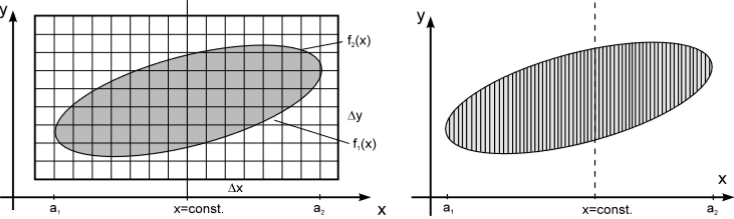
\includegraphics[width= \textwidth]{../pictures/Gebietsintegrale.png}
\caption{Gebietsintegrale}\label{fig:Gebietsintegrale}

\begin{itemize}
	\item es ist egal, ob zuerst nach $x$ oder $y$ integriert wird (wählen was einfacher ist).
	\item Bei Integration nach y: $y(x)$ für die Obere- und Untere- Begrenzungsfunktion berechnen.
	\item nach y integrieren. Mit dem somit berechneten Integral wird die \grqq Strichlänge \grqq{} (eigentlich die Fläche zwischen der $x/y$ Ebene und dem Strich) abhängig von x berechnet.
	\item Von $a_1$ bis $a_2$ über $x$ integrieren. (wird zuerst nach $x$ integriert, $x$ und $y$ jeweils vertauschen)
\end{itemize}

\section{Koordinatensysteme}
\textbf{Schwerpunkt berechnen:} $R=\int \rho(\vec{r}) \cdot \vec{r}\ dV$

\subsection{Zylinderkoordinaten}
\textbf{Flächenelement:} $dA= r\ d\phi dz $\\
\textbf{Volumselement:} $dV=r\ dr d\phi dz \qquad V_{ges}= \int\limits_{0}^{h}\int\limits_{0}^{2\pi}\int\limits_{0}^{r} r\ dr d\phi dz$\\
$\rho = r$

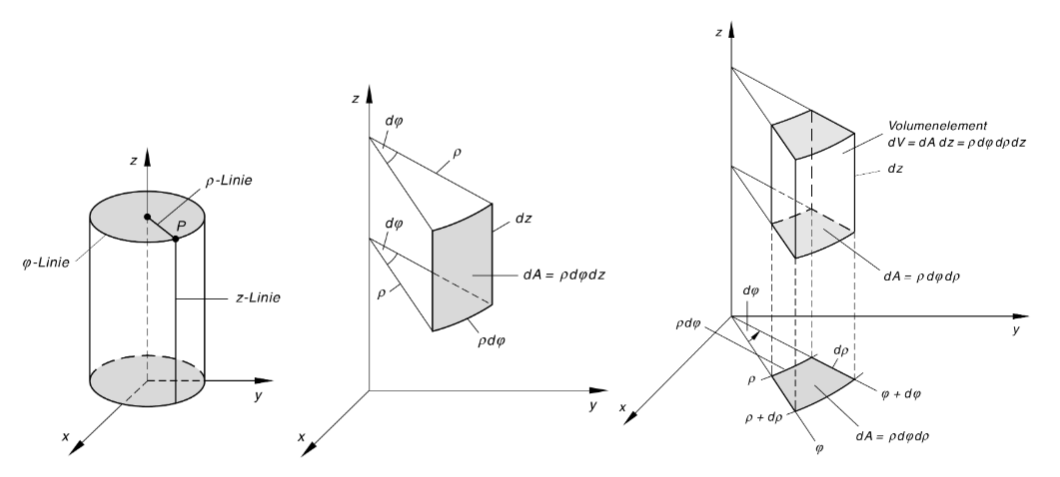
\includegraphics[width=\textwidth]{../pictures/Zylinderkoordinaten.png}

\subsection{Kugelkoordinaten}
\textbf{Flächenelement:} $dA=r^2 \cdot sin \vartheta \ d\vartheta d\varphi \qquad A_{ges} = \int\limits_{0}^{2\pi} \int\limits_{0}^{\pi} r^2\cdot sin\theta \ d\theta d\varphi$\\
\textbf{Volumselement:} $dV= dAdr =r^2 \cdot sin \vartheta \ dr d\vartheta d\varphi \qquad V_{ges} = \int\limits_{0}^{2\pi} \int\limits_{0}^{\pi} \int\limits_{0}^{r}r^2\cdot sin\theta \ dr d\theta d\varphi$

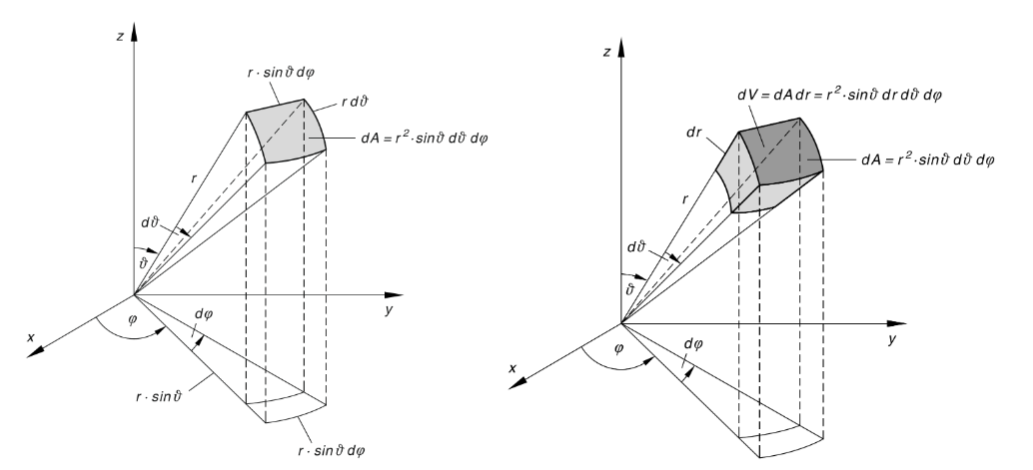
\includegraphics[width=.8\textwidth]{../pictures/Kugelkoordinaten.png}


\textbf{Schwerpunkt berechnen:} $R=\int \rho(\vec{r}) \cdot \vec{r}\ dV = \int\limits_{0}^{2\pi} \int\limits_{0}^{\pi} \int\limits_{0}^{r} \rho(\vec{r}) \cdot \vec{r}\ dr d\theta d\varphi$

\section{Differentialgleichungen}
\textbf{Definition Differentialgleichung:} Eine Gleichung die neben der gesuchten Funktion auch deren Ableitung enthält.\\
\textbf{Gewöhnliche DGL:} Keine partiellen Ableitungen.\\
\textbf{Ordnung:} Höchtse vorkommende Ableitung.\\
\textbf{linear / nicht linear:} nicht linear, wenn die Funktion quadratisch vorkommt.\\
\textbf{homogene DGL:} $y'(x)= h(x)y(x)$\\
\textbf{inhomogene DGL:} $y'(x)= h(x)y(x)+f(x)$\\
\textbf{Ansatz:} Idee zum Lösen einer DGL. Dieser wird in die DGL eingesetzt und anschließend aufgelöst.\\
\textbf{homogene Lösung:} Lösung ohne Störfunktion. ($y_h(x)$) \\
\textbf{partikuläre Lösung:} Lösung mit Störtherm($y_p(x)$) \\
\textbf{allgemeine Lösung:} Lösung der DGL ($y(x)=y_h(x)+y_p(x)$)\\

\textbf{Lösungsverfahren:}
\begin{description}
    \item[Exponentialansatz:] Nur bei \textbf{konstanten Koeffizienten!!}
    \item[Trennen der Variablen:] nur bei \textbf{1. Ordnung.}
    \item[Partikuläre Lösung mit Tabelle:] nur bei \textbf{konstanten Koeffizienten!!}
    \item[Variation der Konstanten:] immer möglich.  
\end{description}

%%
\subsection{Gewöhnliche DGL}
\textbf{implizite Form:} $F(x,y,y',...,y^{(n)})=0$\\
\textbf{explizite Form:} $y^n=f(x,y,y',...,y^{(n-1)})$

%%
\subsubsection{Lösen einer homogenen DGL 1. Ordnung}
$y'(x)=\ga y(x)$
Lösen durch trennen der Variablen oder Exponentialansatz.\\

\textbf{Trennen der Variablen}
\begin{itemize}
    \item $y'$ durch $\frac{dy}{dx}$ ersetzen
    \item alle $y$ und $dy$ sowie $x$ und $dx$ jeweils auf eine Seite bringen.
    \item integrieren
\end{itemize}
$y'(x)=h(x)y(x) \qquad \rightarrow \qquad y(x) = y_0 e ^{\int\limits_{x_0}^{x}h(\tilde{x})d \tilde{x}}$\\

\textbf{Exponentialansatz, nur bei konstanten Koeffizienten!!}\\
$y_0=C\cdot e^{\gl \cdot x}$

\subsubsection{partikuläre Lösung:}

\textbf{mit Tabelle:}
\begin{center}
    \captionsetup{type=figure}
    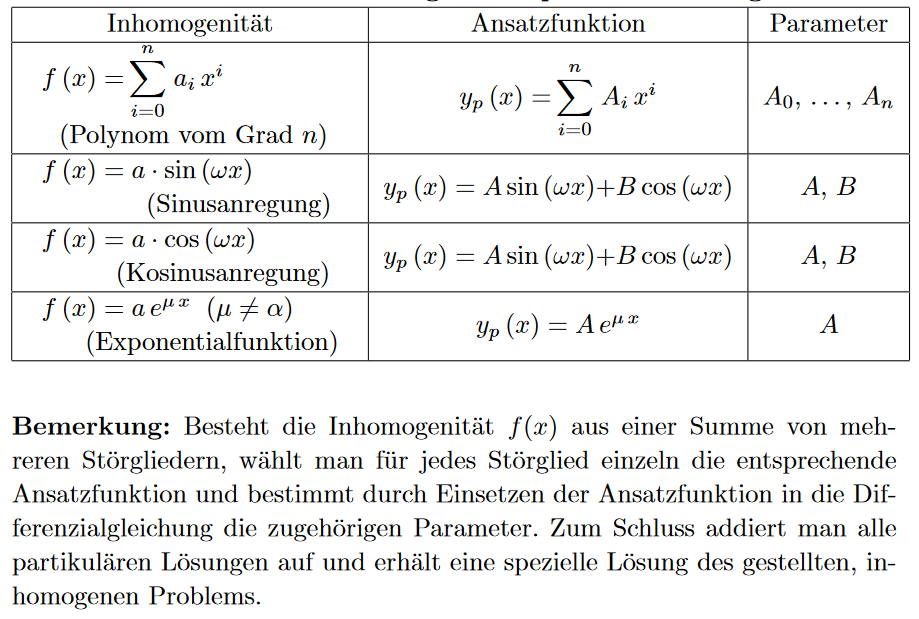
\includegraphics[width=0.9\textwidth]{pictures/Partikuläre_Lösungen_Skript.png}
    \caption{Partikuläre Lösungen}\label{fig:partikuläre_lsg}
\end{center}

Der passende Ansatz wird in die DGL eingesetz und ausgerechnet. Die partikuläre Lösung (bzw. Lösungen bei mehreren Störthermen) werden zur homogenen Lösung addiert und man erhält die Lösung der DGL.\\

\textbf{durch Variation der Konstanten:}
 \[y'(x)=h(x)y(x) + f(x)\]


Berechnen des zugehörigen homogenen Problems $y(x)=C \cdot e ^{\int\limits_{x_0}^{x}h(\tilde{x})d \tilde{x}}$.\\
Die Konstante $C$ wird als variabel $C(x)$ angesehen und der Rest der homogenen Lösung wird $\varphi (x)=e ^{\int\limits_{x_0}^{x}h(\tilde{x})d \tilde{x}}$ geschrieben\\

Es ergibt sich der Ansatz: $\bm{ y(x)=c(x)\cdot \varphi(x)}$, achtung! das ist die \textbf{allgemeine} Lösung\\

Durch Einsetzen von $y(x)$ in die DGL kann man zeigen:

\[c'(x)=\frac{f(x)}{\varphi(x)}\]

somit ist $\bm{c(x) = c_0 + \int\limits_{x_0}^x\frac{f(\tilde{x})}{\varphi(\tilde{x})}d\tilde{x}}$ mit $c_0 = y_0$. 

Eingesetzt in $y(x)$:

\[
    y(x) = \varphi(x) \cdot \left( y_0+\int\limits_{x_0}^x\frac{f(\tilde{x})}{\varphi(\tilde{x})}d\tilde{x}\right)
\]

\subsection{exakte DGL}
Eine DGL 1. Ordnung vom Typ $g(x,y)dx + h(x,y)dy = 0$ ist genau dann \textbf{exaxt}, wenn die Bedingung $\frac{\partial g(x,y)}{\partial y} = \frac{\partial h (x,y)}{\partial x}$ erfüllt ist.\\

Dann ist: $\bm{g(x,y) = \frac{\partial u}{ \partial x}}$ und $\bm{h(x,y) = \frac{\partial u}{ \partial y}}$\\

Durch unbestimmte Integration lässt sich $u(x,y)$ gewinnen, welche in impliziter Form als $u(x,y) = \text{const.} = C$ dargestellt werden kann.\\

$g(x,y)$ muss nach x integriert werden, wobei sich eine Integrationskonstante $K(y)$ ergibt. Um die Integrationskonstante zu bestimmen muss $u(x,y)$ nach $y$ abgeleitet und mit $h(x)$ gleichgesetzt werden. Dann kann $K(y)$ durch integration bestimmt werden. $u(x,y)$ bildet die implizite Lösung und ist konstant ($U(x,y) = \text{const.} = C_2$). Um die explizite Lösung zu erhalten, muss die implizite Lösung $u(x,y) = C_2$ nach $y$ aufgelöst werden.\\

\textbf{Lösen einer exakten DGL:}
\begin{itemize}
    \item $g(x,y)$ nach $x$ integrieren, Integrationskonstante: $K(y)$
    \item $g(x,y)$ nach $y$ ableiten und mit $h(x,y)$ gleichsetzen und damit $K'(y)$ bestimmen
    \item $K(y)$ durch integrieren bestimmen
    \item $u(x,y)$ ist die \textbf{implizite Lösung} der DGL
    \item $u(x,y) = C_2$ nach $y$ auflösen --> \textbf{explizite Lösung!}
\end{itemize}

\subsection{DGL 2. Ordnung}

Wenn die DGL linear ist, ist eine Kombination der Lösung durch Addition auch wieder eine Lösung.

Ansatz: $y_0=C\cdot e^{\gl \cdot x}$

\textbf{homogene Lösung} (Skript 2022x12x07 Seite 8)
\begin{itemize}
    \item Ansatz in DGL einsetzen. Dabei die DGL als homogen behandeln.
    \item $C\cdot e^{\gl \cdot x}$ herausheben. Der Rest bildet das charakteristische Polynom.Dieses 0 setzen.
    \item Alle Nullstellen eingesetzt in den Ansatz sind Lösungen der DGL. Die einzelnen Lösungen können linear kombiniert werden, sprich jede Addition von Lösungen ist wieder eine Lösung der DGL. Die \textbf{allgemeine homogene} Lösung ist die Summe der Lösungen, multipliziert mit Konstanten (nur bei linearen DGL). Durch geschicktes Kombinieren von Komplexe Lösungen können reell konstruiert werden.
\end{itemize}

\textbf{partikuläre Lösung}
\begin{itemize}
    \item Partikuläre Lösung von f(x) mit Tabelle bilden.
    \item Homogene und partikuläre Lösung addieren.    
\end{itemize}




\subsection{LDGL, lineare Differenzialgleichungssysteme erster Ordnung mit konstanten Koeffizienten}

\[ \vec{y}´(t)=A\cdot\vec{y}(t) + \vec{f}(t)\]

mit: $I$... Intervall $\vec{f}(t)=\left(
    \begin{array}{r}
        f_1(t)\\
        \vdots\\
        f_n(t)\\
    \end{array} \right) : I \rightarrow \mathbb{R}^n$, $A$... $n\times n$ Matrix.\\
    Ist $f_i(t) = 0$ wird die LDGDL als homogen bezeichnet.



\begin{itemize}
    \item Eigenwerte von A
    \item Eigenvektoren von A
    \item Fundamentalsystem
    \item homogene Lösung
    \item partikuläre Lösung
\end{itemize}




\newpage
\section{Matritzen}

\textbf{lineare Abhängig:} Eine Zeile einer Matrix ist das Vielfache einer Anderen.\\

\subsection{Determinante}
\[A=\begin{pmatrix}
 a_1 & b_1 \\
 a_2 & b_2 \\
\end{pmatrix}\qquad \text{det}(A)=a_1 \cdot b_2 - a_2 \cdot b_1\]
\ \\
\[A=\begin{pmatrix}
 a_1 & b_1 & c_1 \\
 a_2 & b_2 & c_2 \\
 a_3 & b_3 & c_3 \\
\end{pmatrix}
\begin{matrix}
 a_1 & b_1 \\
 a_2 & b_2 \\
 a_3 & b_3 \\
\end{matrix}\]
\ \\
\[\text{det}(A)= + a_1 \cdot b_2 \cdot c_3 + b_1 \cdot c_2 \cdot a_3 + c_1 \cdot a_2 \cdot b_3 - a_3 \cdot b_2 \cdot c_1 - b_3 \cdot c_2 \cdot a_1 - c_3 \cdot a_2 \cdot b_1\]
\ \\
\textbf{Regel von Sarrus:} Diagonalen miteinander multiplizieren und anschließend summieren. Geht nur bei 3x3 Matrix.\\

\textbf{Rechenregeln zur Determinante:}\\
$z_1,...,z_n$ ... Zeilen, $s_1,...,s_n$... Spalten der Matrix
\begin{itemize}
    \item $\det(s_1,s_2,s_3) = (-1)\cdot \det (s_1,s_3,s_2) = \det(s_3,s_1,s_2)$\\
    werden zwei Zeilen/Spalten vertauscht, muss die Determinante mit $(-1)$ multipliziert werden.
    \item Addition des Vielfachen einer zeile/Spalte zu einer Anderen ändert den Wert nicht.
    \item $\det(k\cdot z_1,z_2,z_3)^T = k \cdot \det(z_1,z_2,z_3)^T \qquad \det(k\cdot a) = k^3\cdot  \det(A)$
    \item $\det(A^{-1} = \frac{1}{\det(A)})$
    \item $\det(A^k) = (\det(A))^k$
    \item $\det(A\cdot B) = \det (A)\cdot \det(B)$
    \item Beil linearer Abhängigkeit ist die Determinante 0
    \item $\bm{\vec{a}\cdot (\vec{b}\times \vec{c})=\det(\vec{a}, \vec{b}, \vec{c})}$
\end{itemize}

\subsubsection{Laplace´scher Entwicklungssatz:}

\[
\text{det}\ A=\sum\limits_{j=1}^{n}(-1)^{i+j}\cdot a_{ij}\cdot \text{det}\ A'_{ij}\qquad \text{für ein festes}\ i\text{ oder } j \in \{1,\ldots,n \}
\]

Die Determinante ändert sich nicht, wenn zu einer Zeile/Spalte ien Vielfaches einer anderen Zeile/Spalte hinzu addiert. Mit dieser Methode versucht man möglichst viele Nullen in eine Zeile/Spalte, nach der man dann die Determinante entwickelt, bekommt.\\

\textbf{Gausß-Jordan-Verfahren:} Beschreibt die elementare Zeilenumformung zum Vereinfachen der Matrix um das Berechnen der Determinante zu erleichtern. Dazu dürfen ganze Zeilen oder Spalten mit einem Faktor multipliziert werden. Weiters dürfen Vielfache von Zeilen/Spalten zu anderen Zeilen/Spalten addiert werden. Wenn zwei Zeilen/Spalten vertauscht werden, ändert sich das Vorzeichen der Determinante.

\subsection{Matrix Multiplikation}

\[A=\begin{pmatrix}
 a_1 & b_1 \\
 a_2 & b_2 \\
\end{pmatrix} \qquad
B=\begin{pmatrix}
 c_1 & d_1 \\
 c_2 & d_2 \\
\end{pmatrix}\]

\[A\cdot B = 
A=\begin{pmatrix}
 a_1 \cdot c_1 + b_1 \cdot c_2 & a_1 \cdot d_1 + b_1 \cdot d_2 \\
 a_2 \cdot c_1 + b_2 \cdot c_2 & a_2 \cdot d_1 + b_2 \cdot d_2 \\
\end{pmatrix}\]\\

\begin{align}
    k*A*x*B &= k*x*(A*B) \qquad \text{ mit } k,x \text{ Konstanten, }A,B \text{ Matritzen}\\
    A\cdot \vec{b} &= \vec{c} \leftrightarrow \vec{b} = A^{-1}\vec{c}    
\end{align}


\subsection{Invertieren einer Matrix}
\begin{boxedminipage}{\textwidth}
    \textbf{Invertieren einer Matrix mit Gauß-Jordan-Verfahren}
    \begin{itemize}
        \item Eine Matrix ist invertierbar, wenn sie
        \item - quadratisch ist
        \item - und die Determinante $\neq$ 0 ist.
    \end{itemize}
\end{boxedminipage}
\ \\

Neben die Matrix wird die Einheitsmatrix geschrieben

\[\left (
    \begin{array}{rrr}
        a_1 & b_1 & c_1 \\
        a_2 & b_2 & c_2 \\
        a_3 & b_3 & c_3 \\
    \end{array}
    \right .
    \left |
    \begin{array}{rrr}
        1 & 0 & 0 \\ 
        0 & 1 & 0 \\
        0 & 0 & 1 \\ 
    \end{array} \right )\]

Die Matrix wird solange mit elementarer Zeilenumformung umgeformt, bis auf der linken Seite die Einheitsmatrix steht (Gauß-Jordan-Verfahren). \\

\textbf{elementare Zeilenumforumengen:}  
\begin{itemize}
    \item Vertauschen von zwei Zeilen
    \item Multiplikation einer Zeile mit $k \neq 0$
    \item Addition des Vielfachen eriner Zeile zu einer anderen
\end{itemize}



\subsection{Wichtige Identitäten}
\begin{center}
    \begin{tblr}{c}
        Identität \\ \hline[1.5pt]
        det $(A^{-1})= \frac{1}{\text{det}(A)}$\\ \hline
        $(A^{-1})^{-1} = A$ \\ \hline
        $(A\cdot B)^{-1}=B^{-1}\cdot A^{-1}$ \\ \hline 
        $(A^t)^{-1}=(A^{-1})^t$ \\ \hline
        $A\cdot A^{-1}=A^{-1}\cdot A=I_n$ \\ \hline 
        $\vec{a}\cdot (\vec{b}\times \vec{c})=\det(\vec{a}, \vec{b}, \vec{c})$\\ \hline
    \end{tblr}
\end{center}



\subsection{Lösungsverfahren:}
\subsubsection{Gaußsches Eliminationsverfahren:}

$\mathbf{A}\cdot \vec{x} =\vec{b}\qquad\rightarrow \qquad \left (\mathbf{A} \left | \vec{b}\right ) \right .$

Soll $\vec{x}$ berechnet werden, wird eine Matrix der Form $(\mathbf{A}|\vec{b})$ aufgeschrieben und solange mit elementarer Zeilenumformung umgeformt, bis über oder unter der Hauptdiagonale von A nur nullen stehen. Mit dem wissen dass die n-te Spalte der Matrix mit $x_n$ multipliziert wird, kann in die erste/letzte Zeile eingesetzt werden.


\subsubsection{Cramersche Regel:}
Sei $A=(a_{ij})$ eine $n\times n$ - Matrix mit den Spaltenvektoren $(a^1,a^2,...,a^n)$ und $\text{det}A\neq 0$. Dann ist die Lösung des LGS
\[a\cdot x = b \qquad \text{mit} \qquad x = (x_1, ... , x_n)^T, b=(b_1,...,b_n)^T\]
gegeben durch
\[x_i=\frac{\text{det}(a^1,...a^{i-1}, b, a^{i+1},...,a^n)}{\text{det}A}\]

Man ersetz die $i$-te Spalete von $A$ durch die Lösung $b$ des LGS. Dann ist $x_i$ der Quotient der so entstandenen Matrix und det$A$.

\subsection{Eigenwertproblem}
$A$... Matrix, $\vec{v}$... Vektor, $k$... Konstante, $I$... Einheitsmatrix\\
\[\textbf{Eigenwertproblem:}\quad \begin{aligned}
    &A\cdot \vec{v} = k \cdot \vec{v}\\
    &A\cdot v - \lambda \cdot v = 0\\
    & (A-\lambda I)\cdot v = 0 \\
\end{aligned}
\]

Jeder Vektor $\vec{v}$ welcher diese Gleichung erfüllt, ist ein Eigenvektor von $A$.\\

\textbf{charakteristisches Polynom:}
$P(\lambda) = \text{det}(A-\lambda I)$\\

\textbf{Eigenwerte:} $P(\lambda) \stackrel{!}{=} 0$ \qquad Nullstellen des charakteristischen Polynoms sind die Eigenwerte der Matrix $A$.\\

\textbf{Eigenvektor:} $\text{Eig}(A, \lambda_i):(A-\lambda_i I)\cdot \vec{x} = 0$
mit $\vec{x} = \begin{pmatrix}
    x_1\\
    x_2\\
    x_3\\
\end{pmatrix}$\\
Die Gleichung nach $x_1,x_2,...1$ auflösen, dann kann der Eigenvektor in Form \\
\[\text{Eig}(A,\lambda_i)= \left\{ \vec{x} \in \mathbb{R}^3 : \vec{x} = r \cdot
\begin{pmatrix}
    x\\
    y\\
    z\\
\end{pmatrix} ; x \in \mathbb{R} \right\}\]
geschrieben werden.

\subsubsection{Herleitung:}
Gibt es nun eine Zahl $\lambda$ und einen Vektor v, sodass dieser durch Multiplikation mit der Matrix $\left(A-\lambda I_n\right)$ auf den Nullvektor abgebildet wird, so ist diese Matrix nicht von vollem Rang und die Multiplikation mit einem Vektor nicht injektiv . Dass die Matrix $\left(A-\lambda I_n\right)$ keinen vollen Rang besitzt ist gleichbedeutend damit, dass ihre Determinante Null ist. Wenn es also eine Lösung des Eigenwertproblems gibt, muss gelten:\\

$\mathrm{det}\left(A-\lambda I_n\right)=0$\\



\section{Nabla}
\textbf{Normaleinheitsvektor:} $N = \frac{\nabla\phi(r)}{|\nabla\Phi(r)|}$\\
\textbf{Nabla:} $\bm {\nabla} = \left(\frac{\partial}{\partial x_1}, \frac{\partial}{\partial x_2}, \frac{\partial}{\partial x_3} \right)$

\begin{center}
    \begin{tblr}{| l | l |}
        \hline
        Bedeutung & Berechnung\\ \hline[1.5pt]
        grad$\Phi = \left(\frac{\partial \Phi}{\partial x_1}, \frac{\partial \Phi}{\partial x_2}, \frac{\partial \Phi}{\partial x_3} \right)$ & $\mathbf{\nabla}\Phi$ \\ \hline
        div$\mathbf{A}=\mathbf{\nabla \cdot A} = \mathbf{\nabla \cdot \nabla}\Phi$ & $\mathbf{\nabla\cdot A}$\\ \hline
        rot$\mathbf{A}$ = rot grad$\Phi$ = $\mathbf{\nabla \times \nabla} \Phi$ & $\mathbf{\nabla \times A}$\\ \hline
    \end{tblr}
\end{center}

\textbf{Gradient}\\
Erzeugt ein Vektorfeld mit den Steigungen des skalaren Feldes aus einem skalaren Feld. (Vektor)\\

\textbf{Divergenz}\\
Gibt an ob die Vektoren in diesem Punkt zusammen oder auseinander zeigen. (Skalar)

\begin{itemize}
    \item div$\mathbf{A} > 0A>0$: im Volumenelement befindet sich eine Quelle (mehr raus als rein)
    \item div$\mathbf{A} < 0A<0$: im Volumenelement befindet sich eine Senke (mehr rein als raus)
    \item div$\mathbf{A} = 0A=0$: Im Volumenelement befindet sich weder eine Quelle noch eine Senke, das Vektorfeld ist an dieser Stelle quellenfrei.
\end{itemize}

\textbf{Rotation}\\
Gibt an, ob sich das Vektorfeld um einen Punkt dreht. (Vektor)

%%% Verzeichnisse
\newpage
%\listoftables
%\listoffigures
\printbibliography{}
%%%%%% Document end
\end{document}     %%% End the document
